% Editable Overleaf report. Compile main.tex using pdfLaTeX.
\documentclass[10pt,letterpaper]{article}
\usepackage[margin=.70in]{geometry}
\usepackage[T1]{fontenc}
\usepackage{mathpazo,graphicx,booktabs,tabularx,array,amsmath,xcolor,fancyhdr,enumitem,hyperref,microtype}
\usepackage{tikz,helvet}
\usetikzlibrary{arrows.meta}
\definecolor{ink}{HTML}{173247}\definecolor{accent}{HTML}{007D9D}\definecolor{muted}{HTML}{536775}
\hypersetup{colorlinks=true,urlcolor=accent,linkcolor=accent}
\setlength{\parindent}{0pt}\setlength{\parskip}{5pt}
\setlist[itemize]{leftmargin=*,nosep,topsep=3pt}
\pagestyle{fancy}\fancyhf{}\fancyhead[L]{\small\textcolor{muted}{Arm26 | Adaptive control progress update}}\fancyhead[R]{\small Hussein Zolfaghari}\fancyfoot[C]{\small\thepage}\setlength{\headheight}{14pt}
\newcommand{\heading}[1]{\vspace{4pt}{\large\bfseries\color{accent}#1}\par}
\newcommand{\note}[1]{{\small\color{muted}#1}\par}
\newcolumntype{Y}{>{\raggedright\arraybackslash}X}
\begin{document}
{\Large\bfseries Adaptive PI--NN Control with EWC-Inspired Regularization}\par
{\large Tracking under changing dumbbell loads}\par
\textcolor{muted}{Technical progress update | Recorded run: \texttt{2026-10-18\_14-43-00\_UTC\_5b5dfe48}}

\heading{1. Question and implemented controller}
The objective is to adapt elbow tracking to changing load while retaining useful learned compensation. A proportional--integral (PI) controller is augmented with fixed proportional--derivative (PD) assistance and a learned residual torque. The adaptive correction uses a memory penalty inspired by \textbf{elastic weight consolidation (EWC)}. We call this the \textbf{adaptive (EWC-inspired) controller}. Learning changes \textbf{32 basis coefficients}; it does not tune the PI gains.\par
\centerline{\resizebox{\linewidth}{!}{% Editable vector control diagram. Solid: signal/actuation; dashed blue: weight update.
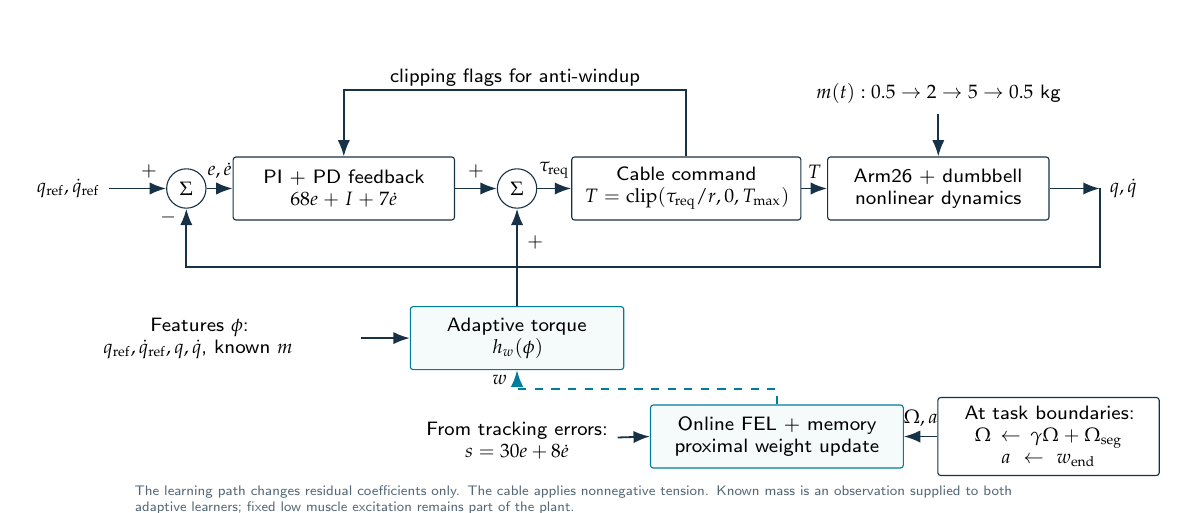
\begin{tikzpicture}[>=Latex,font=\sffamily\scriptsize,
 block/.style={draw=ink,rounded corners=1pt,fill=white,align=center,minimum height=8mm,inner sep=3pt},
 sum/.style={circle,draw=ink,fill=white,inner sep=0pt,minimum size=5mm},
 signal/.style={->,draw=ink,line width=.65pt},
 learn/.style={->,draw=accent,dashed,line width=.7pt}]
\node[align=center] (ref) at (0,0) {$q_{\rm ref},\dot q_{\rm ref}$};
\node[sum] (err) at (1.5,0) {$\Sigma$};
\node[block,text width=26mm] (fb) at (3.5,0) {PI + PD feedback\\$68e+I+7\dot e$};
\node[sum] (torque) at (5.7,0) {$\Sigma$};
\node[block,text width=27mm] (cable) at (7.85,0) {Cable command\\$T=\mathrm{clip}(\tau_{\rm req}/r,0,T_{\max})$};
\node[block,text width=26mm] (plant) at (11.05,0) {Arm26 + dumbbell\\nonlinear dynamics};
\coordinate (out) at (13.1,0);
\draw[signal] (ref) -- node[above,pos=.7] {$+$} (err);
\draw[signal] (err) -- node[above] {$e,\dot e$} (fb);
\draw[signal] (fb) -- node[above] {$+$} (torque);
\draw[signal] (torque) -- node[above] {$\tau_{\rm req}$} (cable);
\draw[signal] (cable) -- node[above] {$T$} (plant);
\draw[signal] (plant) -- (out) node[right] {$q,\dot q$};
\draw[signal] (out) -- (13.1,-1.0) -- (1.5,-1.0) -- node[left,pos=.85] {$-$} (err.south);
\node[above] (load) at (11.05,.95) {$m(t):0.5\to2\to5\to0.5$ kg};
\draw[signal] (load) -- (plant.north);
\draw[signal] (cable.north) -- (7.85,1.25) -- node[above,fill=white,inner sep=1pt] {clipping flags for anti-windup} (3.5,1.25) -- (fb.north);
\node[block,text width=25mm,draw=accent,fill=accent!4] (nn) at (5.7,-1.9) {Adaptive torque\\$h_w(\phi)$};
\draw[signal] (nn.north) -- node[right,pos=.65] {$+$} (torque.south);
\node[align=center,text width=39mm] (features) at (1.65,-1.9) {Features $\phi$:\\$q_{\rm ref},\dot q_{\rm ref},q,\dot q$, known $m$};
\draw[signal] (features) -- (nn);
\node[block,draw=accent,fill=accent!4,text width=30mm] (update) at (9,-3.15) {Online FEL + memory\\proximal weight update};
\node[block,text width=26mm] (memory) at (12.45,-3.15) {At task boundaries:\\$\Omega\leftarrow\gamma\Omega+\Omega_{\rm seg}$\\$a\leftarrow w_{\rm end}$};
\draw[signal] (memory) -- node[above] {$\Omega,a$} (update);
\draw[learn] (update.north) -- (9,-2.55) -- (5.7,-2.55) -- node[left] {$w$} (nn.south);
\node[align=center] (teacher) at (5.7,-3.2) {From tracking errors:\\$s=30e+8\dot e$};
\draw[signal] (teacher) -- (update.west);
\node[below,align=left,text width=115mm,font=\sffamily\tiny,text=muted] at (6.6,-3.65) {The learning path changes residual coefficients only. The cable applies nonnegative tension. Known mass is an observation supplied to both adaptive learners; fixed low muscle excitation remains part of the plant.};
\end{tikzpicture}
}}\par
\note{Control configuration: solid arrows carry signals/actuation; the dashed blue arrow updates neural coefficients. The outer loop uses measured angle/speed; the lower path is online learning.}
\begin{equation}
\tau_{\rm req}=30e+I+38e+7\dot e+h_w(\phi),\quad
T=\operatorname{clip}\!\left(\frac{\tau_{\rm req}}{r(q)},0,T_{\max}\right).
\end{equation}
Here $e=q_{\rm ref}-q$ is angle error (rad), $\dot e$ is speed error (rad/s), $I$ is integral torque (N\,m), $r(q)$ is moment arm (m), and $T$ is cable tension (N). The adaptive branches use $\dot I=5.25e$ when anti-windup permits integration. The fixed-PI baseline uses $\dot I=15e$ and no added PD term; it is a contextual baseline, not the matched EWC ablation.

The residual is $h_w=45\tanh(w^\top\phi/45)$ N\,m. Features include reference-angle Gaussian functions, trigonometric/speed terms, and known mass modulation. The two new adaptive branches use the same features and feedback gains.

\heading{2. What loss/update is actually implemented?}
The learning signal is $s_k=30e_k+8\dot e_k$. Holding the current state and features fixed, the un-clipped feedback-error learning (FEL) surrogate is $\ell_k(w)=-s_kh_w(\phi_k)$. This is \textbf{not} backpropagation of tracking mean squared error through OpenSim. With $d_k=\operatorname{clip}(s_k\nabla_wh_w, -25,25)$ and $\alpha=0.95\Delta t$, the implemented step minimizes the local quadratic objective
\begin{equation}
\mathcal Q_k(w)=-d_k^\top(w-w_k)+\frac{\|w-w_k\|^2}{2\alpha}
+\underbrace{\frac{\lambda}{2}\sum_i\Omega_i(w_i-a_i)^2}_{R(w):\ \text{memory penalty}},
\quad
w_i^+=\frac{w_{i,k}+\alpha d_{i,k}+\alpha\lambda\Omega_i a_i}{1+\alpha\lambda\Omega_i}.
\end{equation}
$w$ denotes learned coefficients, $a$ the latest segment-end anchor, and $\Omega$ accumulated squared-output-sensitivity importance. Here $\lambda=5$. This proximal step avoids the isolated explicit quadratic-penalty step restriction. A tracking diagnostic, $\tfrac12e^2$, is plotted separately; it is not the training objective differentiated through the plant.

\note{Terminology: this is EWC-inspired sensitivity regularization. A tracking-likelihood Fisher estimate and frozen-task retention benefit have not yet been established. Bounded output and a stable penalty step do not by themselves prove closed-loop stability.}



\newpage
\heading{3. Full comparison and the heavy-load interval}
The same 65.5 s motion contains eight $20^\circ\!\to80^\circ\!\to20^\circ$ cycles. Mass changes $0.5\to2\to5\to0.5$ kg at 16.5, 32.5 and 48.5 s. Control interval is 0.01 s, and all methods use the same 240 N cap. Physical/muscle states and integral torque carry through ideal no-impact exchanges.

\IfFileExists{figures/video_preview.png}{
\centerline{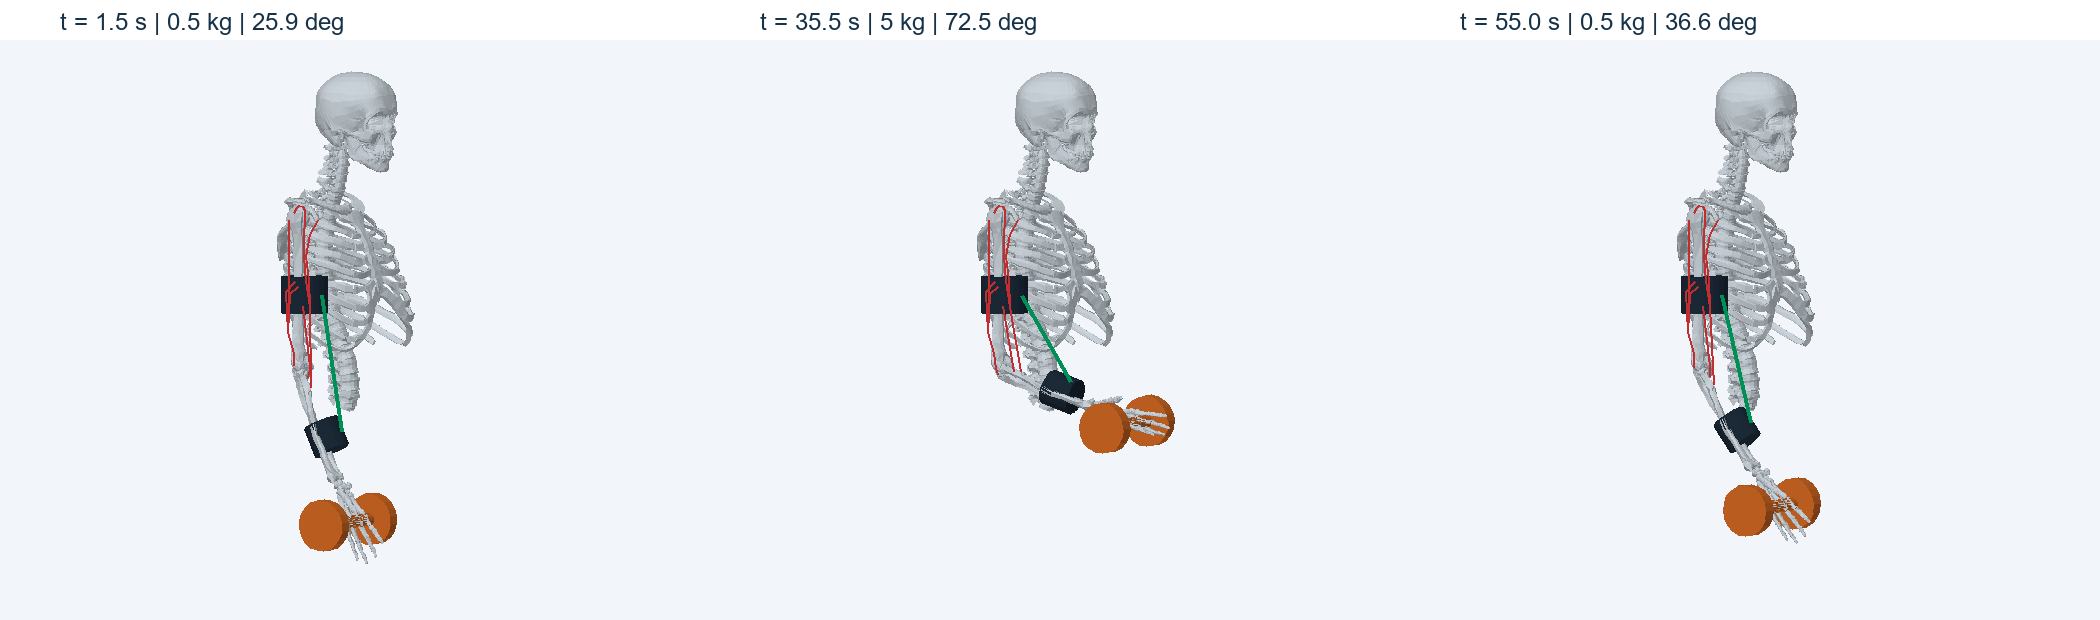
\includegraphics[width=\linewidth,height=1.0in,keepaspectratio]{figures/video_preview.png}}\par
\note{Figure 1. Frames from the actual recorded-state replay. Bone meshes and muscle/cable paths are transformed using OpenSim states. This is a rendered replay, not a desktop recording. Mass changes physically during simulation; dumbbell dimensions stay fixed.}}

\centerline{\includegraphics[width=\linewidth,height=3.70in,keepaspectratio]{figures/tracking_comparison.pdf}}\par
\note{Figure 2. All controller scenarios together: load, trajectory, error, applied tension and learned-only torque. The large heavy-load oscillation belongs to fixed PI. The updated adaptive controller tracks with 0.651$^\circ$ heavy-load RMSE and 0.658$^\circ$ overall RMSE. The updated controller does not clip its command in this recorded run.}

\centerline{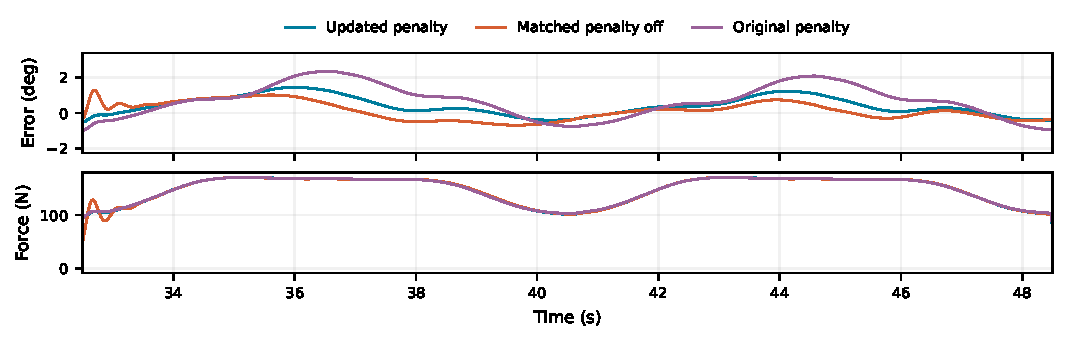
\includegraphics[width=\linewidth,height=2.0in,keepaspectratio]{figures/heavy_load_zoom.pdf}}\par
\note{Figure 3. Adaptive methods at 5 kg. Updated error is lower than the original penalty controller (1.130$^\circ$ RMSE). The matched penalty-off learner remains a strong comparator (0.510$^\circ$). The baseline remains visible in Figure 2.}

\newpage
\heading{4. Controller, muscle and learning diagnostics}
\centerline{\includegraphics[width=\linewidth,height=4.00in,keepaspectratio]{figures/simulation_dashboard.pdf}}\par
\note{Figure 4. Saved six-panel dashboard for the updated controller. Learned torque is separated from fixed PD assistance and integral torque. Fiber lengths and tendon forces vary with movement; all six muscles receive fixed 0.01 excitation, so these traces do not show learned voluntary muscle recruitment or reduced biological effort.}

\centerline{\includegraphics[width=\linewidth,height=3.00in,keepaspectratio]{figures/learning_diagnostics.pdf}}\par
\note{Figure 5. Top: tracking diagnostic $\tfrac12 e^2$ (rad$^2$). Middle: the local FEL surrogate $-s_kh_w$, which may be negative and need not decrease monotonically along changing states/tasks. Bottom: recorded memory penalty before updates. The final penalty point is omitted because no learning update is taken at the terminal sample. These quantities have different scales and meanings.}

\newpage
\heading{5. Stored memory and quantitative results}
\centerline{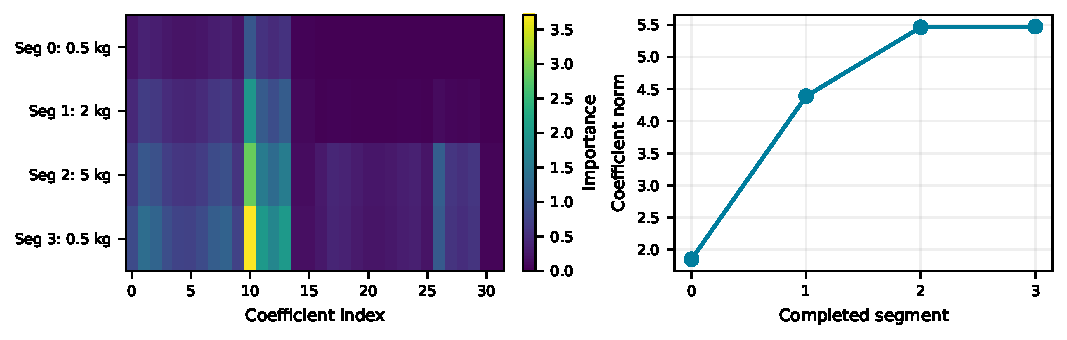
\includegraphics[width=\linewidth,height=2.50in,keepaspectratio]{figures/memory_diagnostics.pdf}}\par
\note{Figure 6. Importance at task boundaries and coefficient norm. This verifies that the algorithm records parameter information. It does not establish that an earlier task is remembered; that requires a separate performance evaluation with learning frozen. Importance is a normalized sensitivity proxy, not a proven Fisher estimate for tracking loss.}

\small
\begin{tabularx}{\linewidth}{@{}Yrrrrr@{}}\toprule
\textbf{Controller} & \textbf{0.5 kg} & \textbf{2 kg} & \textbf{5 kg} & \textbf{Return} & \textbf{Overall}\\\midrule
Adaptive (EWC-inspired) & 0.456 & 0.998 & 0.651 & 0.358 & 0.658\\
Matched penalty off & 0.456 & 0.470 & 0.510 & 0.843 & 0.595\\
Original penalty learner & 0.456 & 1.431 & 1.130 & 0.914 & 1.040\\
Fixed PI baseline & 2.754 & 4.425 & 9.814 & 4.628 & 5.981\\
\bottomrule
\end{tabularx}
\note{RMSE in degrees. These are actual computed simulation results, not target curves inserted as outputs. All cases completed; 6,551 samples per case. The return column scores active learning and load-transition response; it is not an isolated forgetting measurement.}
\normalsize

\heading{What can be concluded now?}
\begin{itemize}
\item \textbf{Tracking:} updated heavy-load RMSE is 0.651$^\circ$, versus 1.130$^\circ$ for the earlier penalty controller. The new adaptive pair keeps the same gains, features, reference and force cap.
\item \textbf{Trade-off:} the penalty-off learner achieves 0.595$^\circ$ overall RMSE, compared with 0.658$^\circ$ for the updated penalty learner. On this sequence, return-segment error is 0.358$^\circ$ versus 0.843$^\circ$. Neither score proves a general memory advantage.
\item \textbf{Update changes:} the old explicit step and selective anchors were replaced with a proximal step and a latest-endpoint anchor; $\lambda$ is 5 (previously 95). Numerical stabilization alone barely changed heavy-load RMSE in the diagnostic test; weakening protection permits more new-load adaptation.
\end{itemize}

\heading{Relationship to the reference paper and next test}
Piqu\'e et al. learn an inverse neural controller through a learned forward dynamics model and apply EWC during retraining between trials. Here the PI/PD feedback structure is retained and an output-torque model is updated directly during movement using FEL. The shared idea is protecting learned parameters; the learning objective and adaptation schedule differ.

The next test is to train A--B--C, then \textbf{freeze learning} and evaluate every previous load from the same physical and integral initial states. Use several held-out load orders, paired across penalty-on/off methods. This separates retention from transition dynamics, online relearning and actuator limitations. Current parameters were selected on this schedule; no hardware or generalization claim is made.

\heading{Saved outputs}
Every figure is exported as PNG and vector PDF. Raw controller/muscle signals, diagnostics, task checkpoints and OpenSim motion/state tables are saved. The video is a replay of those states, with time, mass, target, actual angle and force annotated. The accompanying code regenerates the figures, video and this editable Overleaf project for each run.

\vfill
\note{Reference: F. Piqu\'e et al., ``Controlling Soft Robotic Arms Using Continual Learning,'' IEEE RA-L 7(2), 5469--5476 (2022). DOI: \href{https://doi.org/10.1109/LRA.2022.3157369}{10.1109/LRA.2022.3157369}.}
\end{document}
